\glsresetall

\chapter{Virtualização e Migração de Processos em \Lws}
\label{chap.dev.virtualizacao}

Visando aumentar a independência dos processos no processador, este trabalho tem como objetivo o desenvolver o suporte à virtualização e migração de processos em \lws. As características arquiteturais dos \lws, especialmente relacionadas à memória, inviabilizam um suporte complexo para virtualização. Por exemplo, máquinas virtuais utilizadas em ambientes \cloud possuem à disposição centenas de GBs para isolar duplicatas inteiras de \oss com a ajuda de virtualização no nível de instrução~\cite{sharma2016containers}. Nos \lws, as pequenas memórias locais e a simplificação do \hardware para redução do consumo energético restringem os tipos de virtualização suportados nesses ambientes computacionais.
%
Neste contexto, o presente trabalho explora um modelo de virtualização baseado em contêineres adaptado para \lws. Contêineres são executados pelo \os como aplicações virtuais e não incluem um \os convidado, resultando em um menor impacto no sistema de memória e requerendo menor complexidade do \hardware~\cite{thalheim2018cntr, sharma2016containers}.


\begin{figure}[t]
	\centering
	
	\subcaptionminipage[fig.nanvix.without-uarea]%
                   {.4\textwidth}
                   {\os sem isolamento.}
                   {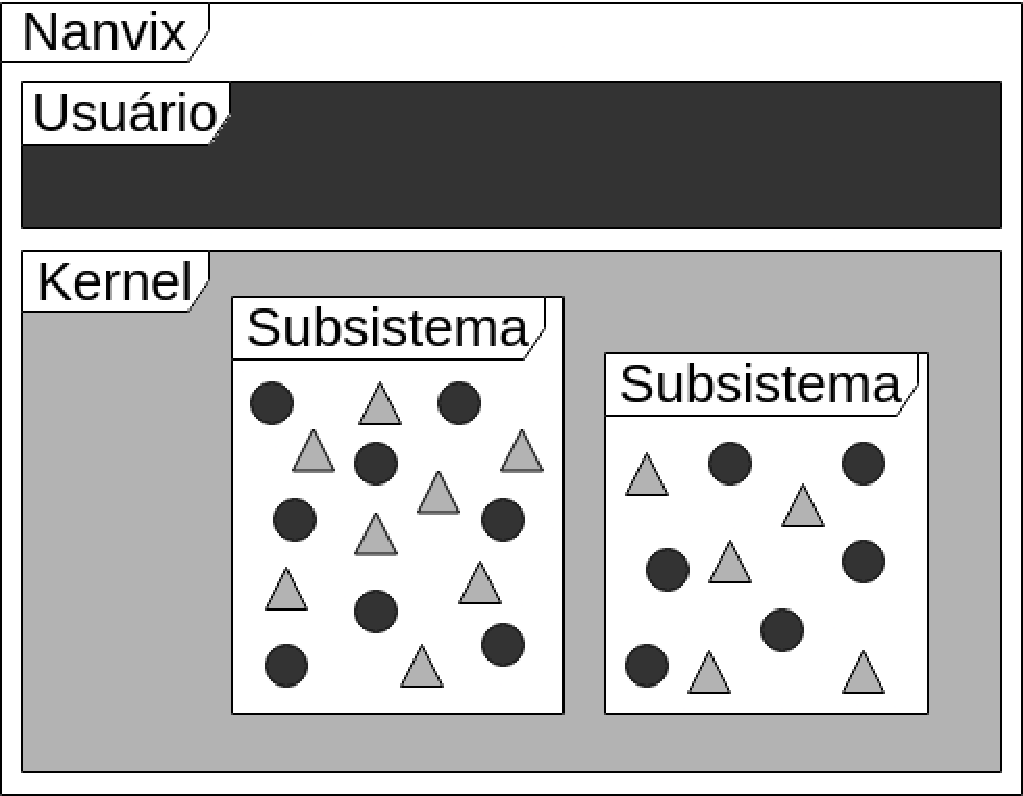
\includegraphics[width=\textwidth]{content/images/nanvix-without-uarea-uk.pdf}}
	\qquad
	\subcaptionminipage[fig.nanvix.with-uarea]
                   {.4\textwidth}
                   {\os com isolamento.}
                   {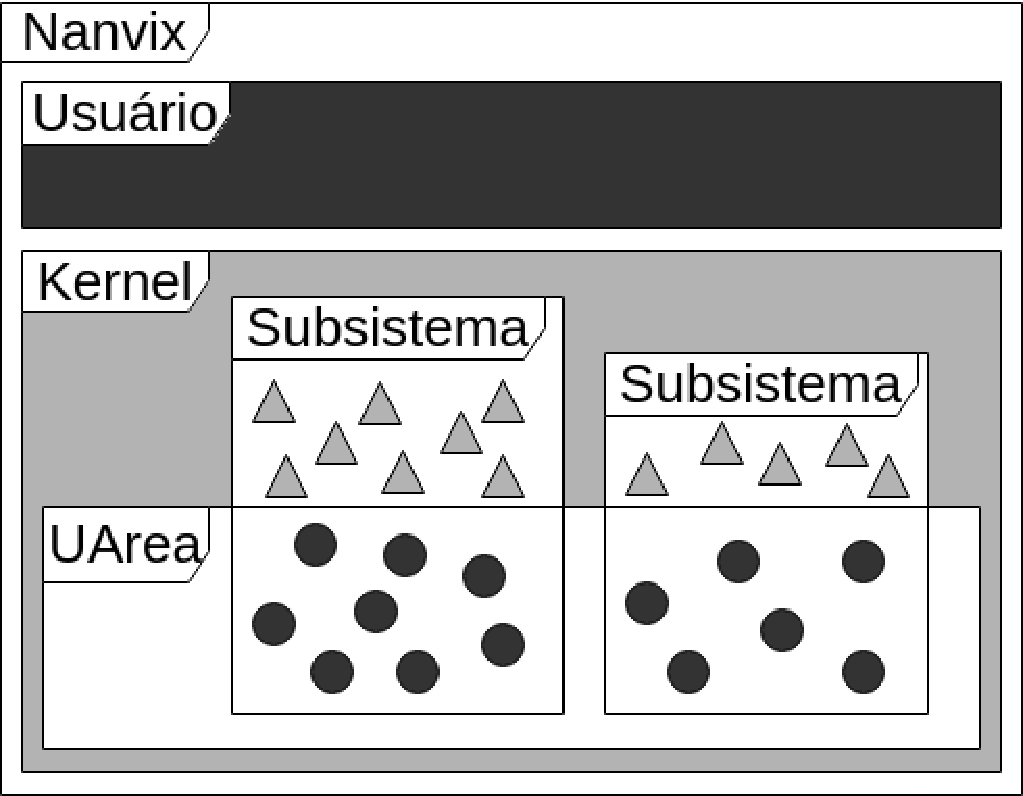
\includegraphics[width=\textwidth]{content/images/nanvix-with-uarea-uk.pdf}}

	
\includegraphics[width=.33\linewidth]{content/images/legenda.pdf}
	
	\caption{Diferença da estrutura do \nanvix com e sem a \textit{User Area}.}%
\end{figure}

\section{Separação Kernel-Usuário}
\label{sec.dev.kernel-usuario}

\subsection{Divisão de Dados e Instruções}
\label{sec.divisao-dados-instrucao}
    Para a virtualização de processos através da conteinerização, é recomendável que as informações relevantes para a manipulação dos processos em execução estejam isoladas das informações internas do próprio \os para que os recursos de \hardware sejam utilizados de maneira eficiente~\cite{choudhary2017critical}.
    A Figura~\ref{fig.nanvix.without-uarea} ilustra como os subsistemas do \nanvix são originalmente estruturados. Não há uma divisão explícita do que são dados para funcionamento interno do \os ou dependências locais do processo.
    Esta abordagem torna algumas das funcionalidades do \os onerosas porque ela dificulta o acesso às informações do processo e impacta partes independentes do sistema, \eg migração e segurança dos processos.

    Durante a geração de um executável no \nanvix, originalmente, após cada arquivo ser compilado separadamente, bibliotecas estáticas eram geradas para cada camada do \nanvix (\hal, \microkernel, \libnanvix, \ulibc e \multikernel). Depois disso, o executável era gerado, utilizando as bibliotecas. O problema disso é que os dados e instruções de \kernel e usuário ficam misturadas nas seções do binário final, não existindo uma separação explícita.

    Sendo assim, visando a separação das informações entre aplicação de usuário e \kernel, o \script de ligação original do \nanvix foi adaptado. Na versão desenvolvida, as seções .text, .data, .bss e .rodata dos arquivos que são compilados são renomeados com a camada na qual este arquivo está incluído. Dessa forma, na montagem no binário final, é possível identificar quais são os dados e instruções de cada camada do \nanvix, bem como identificar as informações de aplicação. Sendo assim, são geradas seções .text, .data, .rodata e .bss específicas para o \kernel e usuário. Portanto, todas as informações de \kernel, alocadas nos endereços mais baixos da memória, são isoladas das informações de aplicação, alocadas nos endereços mais altos da memória. Nesse processo, são exportadas algumas constantes que apontam onde começam e terminam as partes do binário que são relacionadas ao \kernel e à aplicação. Com essas constantes é possível manipular os endereços de aplicação e \kernel com mais precisão.
    
    Através dessa estratégia, todos os \clusters passam a ter a mesma organização interna de \kernel. O que facilita a migração, já que pode-se ''copiar'' os dados e instruções de aplicação de um \cluster e ''colar'' em outro nos mesmos locais, que são identificados pelas constantes exportadas no processo de compilação. Com isso, evita-se manipulações mais complexas do processo como a expansão de várias regiões entre as seções.

    \mytodo{colocar alguma parte do linker?}

\section{\textit{User Area}}
\label{sec.uarea}

    Além da necessidade de separação de dados e instruções de \kernel e aplicação, é necessário a identificação e separação das estruturas internas do \so que são manipuladas pelo usuário. Nesse contexto, é introduzido o conceito de conteinerização. Isso porque as dependências que o usuário possui dentro do \cluster \ie dados que são gerenciados pelo \kernel mas pertencem ao contexto do processo de usuário, são isolados em uma região bem definida da memória, que é chamada de \uarea. 

    Mais detalhadamente, a \uarea mantém informações sobre:
    \begin{enumerate}[label=(\roman*)]
        \item \threads ativas, incluindo identificadores e contextos;
        \item ponteiros para suas pilhas de execução; 
        \item variáveis de controle e filas de escalonamento;
        \item estruturas de gerenciamento de chamadas de sistema;
        \item estruturas de gerenciamento de memória (estado do mapeamento, frames, etc);
    \end{enumerate}

    Essa estrutura foi pensada genericamente para englobar as várias arquiteturas que o \nanvix suporta. Além disso, foi planejada com a possibilidade de expansão, não se limitando ao estado atual do desenvolvimento do \nanvix. Dessa forma, essa estrutura pode ser facilmente expandida ou modificada para atender os objetivos que algum projeto que envolva o \nanvix possa ter.

\section{Migração de Processos}
\label{sec.migracao}

Como aplicação direta do isolamento do processo, a migração de processos torna-se mais eficiente. Com a criação de uma instância isolada do espaço do usuário via conteinerização, eliminamos a necessidade de descobrir quais são e onde estão as dependências do processo, facilitando a transferência de seu contexto.  Isso só é possível porque os \clusters possuem uma estrutura de \kernel idêntica (devido às mudanças desenvolvidas no processo de compilação detalhados na Seção \ref{sec.divisao-dados-instrucao}), descartando a necessidade do envio de dados relacionados ao \os. Ao evitar o envio de dados redundantes entre \clusters, atenuamos o impacto da migração sobre a \noc.

\subsection{Rotina de migração}
\label{sec.rotina-migracao}

Para a migração de um processo entre \clusters foi desenvolvida uma rotina de migração. A funcionalidade é similar ao \criu, ferramenta utilizada por \softwares de gerenciamento de contêineres como o Docker. Porém, a migração será executada por intermédio de \deamons do \os. Trata-se de uma \hotmigration, em que a aplicação é migrada durante sua execução, com cópia das páginas de memória da aplicação.
As próximas seções detalham o fluxo de execução da migração.

\subsubsection{A execução do processo em um \cluster é congelada em um estado consistente}
    Antes do envio do processo a outro \cluster, é necessário que este esteja em um estado consistente e estático. Isso significa que durante o processo de migração é preciso que todas as operações dele sejam pausadas. Isso com o intuito de evitar inconsistências que podem ser causadas por condições de corrida. Para atingir esse estado consistente, a chamada de sistema \freeze é invocada. Esta é uma chamada de sistema que é tratada apenas pelo \mcore de um \cluster. Mais detalhadamente, esta chamada impede o escalonamento de \threads de aplicação \ie \threads que não executam no \mcore. Isso garante uma pausa na aplicação sem que o \so seja impedido de executar no \cluster, o que é imprescindível para a migração, já que as informações do processo precisam ser enviadas das interfaces \noc do \cluster remetente, o que exige que o \so atenda às requisições de envio de dados.

    Após o congelamento da aplicação, são verificados os \buffers de chamadas de sistema. Após o travamento no escalonamento de \threads de usuário, novas chamadas de sistema requisitadas pela aplicação não podem ocorrer. Contudo, a fim de evitar a perda de qualquer chamada que possa ter sido requisitada antes do congelamento do escalonamento, os \buffers de chamada de sistema são verificados várias vezes. Todas as chamadas de sistema vindas de \threads de aplicação que são encontradas, são tradadas antes da migração.

    Após o congelamento do escalonamento e verificação nos \buffers de chamada de sistema, o processo é considerado consistente e seu contexto pode ser migrado.

\subsubsection{O contexto do processo é enviado para outro \cluster}

    Com o processo em um estado consistente, uma \task de sistema, que é executada no \mcore, é criada para o envio dos dados ao \cluster destinatário. Através das abstrações de comunicação \mailbox e \portal, as seções de dados e instruções do processo são enviadas ao \cluster destinatário. Logo após, a \uarea é enviada também. O envio de dados, instruções e \uarea garantem que o contexto inteiro do processo é enviado, possibilitando a retomada da execução no \cluster destinatário.


\subsubsection{A execução do processo é restaurada em outro \cluster}
    Com o contexto do processo já no \cluster destinatário, a execução é restaurada. Isso é feito pela chamada de sistema \unfreeze, que descongela o escalonamento de \threads de usuário. Assim, a execução do processo continua normalmente, agora em outro \cluster.





